
\chapter{Research Background}
	%%%%%%%%%%
	DEFINITIONS DEFINITIONS DEFINITIONS
	\section{Domain}
	%%%%%%%%%%
		%%%%%%%%%%
		\subsection{Business Process Outsourcing}
		%%%%%%%%%%
		The phenomenon of outsourcing can be explained by basic economic theory. The following section describes how the theory of the firm, the value chain, outsourcing and process orientation are interwoven. 
		
		
		\subsubsection{Theory of the Firm}
		In theory, a firm exists because of transaction and production costs efficiencies. They are organizational innovations to reduce costs involved in market transacting. A transaction here means the transfer of a good or service across a technologically separable interface \cite{williamson1981economics, williamson1971vertical}, like the boundaries between firms. If the transaction costs across markets become larger than the costs of managing the firm, firms will substitute market transactions through internal execution. IT has drastically reduced these transaction costs and the IS field is applying transaction cost theory to explain its impact on the boundaries of the firm \cite{aron2005just}.
		The theory of production cost efficiency states that production by multiple individuals is the characteristic of a firm \cite{alchian1972production} and it will exist as long as the output is sufficiently larger than the output under independent production, so that the costs of organizing individuals are justified. What economists describe as increasing returns, \ie, economies of scale or experience, follows a simple rule: the more you do of something, the better you get. \todo{hä?}
		
		As an asset's productivity increases with specialization, this in return explains why firms specialize in certain tasks: costs of managing the firm increase with size,  benefits in productivity are reachable through focusing on their core business.
		When a firm makes its core business to parts that others do not choose to, they can provide these as a service on the market place - and decreasing transaction costs make it more and more attractive to make us of these. \todo{servitization?}
		
		\subsubsection{The value chain}
		Drawing on the concept of the value chain by Porter \cite{porter1985}, the idea is to model each firm as a set of systems, which add value to a product or service. These chains can be concatenated, as more and more actors are involved on the way to the end consumer to make a final product out of raw materials and components. Transaction costs are the glue that hold chains together. Within each chain for a firm lie different subsystems, which contribute to the created value through the consumption of resources - like money, labor or material. Strategy demands that firms build sustainable competitive advantages to be able to survive in the market. As firms cannot build these in all stages of their value chain \cite{Ramachandran2004}, they choose to focus in certain activities and hence invest less resources in others. 
		
		As transaction costs are composed of costs for communication and information processing \cite{evansted}, One can see how digitalization impacts these theories from the last century. Communication costs have fallen faster than processing costs since the mid 90s\todo{SRC}, which is manifested in the internet. With falling costs, value chains can easier break up and be more flexible.
		
		Combining the previously mentioned theories of the firm and the value chain, organizations can easier transfer activities to other actors in the market that have specialized on it and can deliver it better and more efficient.  
		
			\subsubsection{(Business Process) Outsourcing}
		The term outsourcing can be derived from \textbf{out}side re\textbf{sourcing} and dates back to 1981\todo{src}. It can be broadly defined by \enquote{the purchase of a good or service that was previously provided internally} \citep[\p{74}]{lacity1993} or more narrow as \enquote{contracting with an external firm for the ongoing management and delivery of a defined set of services to a prescribed level of performance} \citep[\p{2}]{cohen2006multisourcing} . However, it does not necessarily mean relocating it to a foreign country (offshoring), which falsely gave the term a negative connotation in Germany in the past \footnote{ "Outsourcing" was chosen the Un-word of the year 1996 \url{http://www.unwortdesjahres.net/index.php?id=33}}. Outsourcing can be distinguished by other types of partnerships through a contract that clearly defines subject and duration of the cooperation \todo{src}. 
		
		\cite{Lee:2000} give an overview about theoretical foundations in outsourcing research. Three major views are identified:
		
		\begin{itemize}
			\item Strategic management view
			\item Economic view
			\item Social view
		\end{itemize}
		
		The first builds on the resource based view \cite{wernerfelt1984resource} and takes a merely internal view. Here, the firm's strategy is about its capabilities, captured in scarce resources, and reasons outsourcing to focus on its core competencies. The economic view brings transaction cost theory into play and argues that specialized organizations (outsourcing providers) are able to achieve economies of scale. Lastly, apart from this cost efficiency focus, relationships between provider and client are also an issue worth explaining. Here, social exchange and power political theory \cite{lee1999effect} can be named. This view is justified by the fact that two mechanisms, namely trust and power, are explaining relationships between organizations. These play an important role in establishing and especially maintaining a relationship, which is leveraging economies of scale and scope provided by partnering organizations \cite{rai1996critical}. 
		
		% despite the fact that earlier work in the field \cite{cheon1995theoretical} did not consider it
		
		Processes in which IT plays an important role became prime candidates for outsourcing, as transaction costs for information are negligible. More sharply, one can speak of \acrfull{ITES} that can be outsourced using the power of IT \citep[\p{49}]{Ramachandran2004}. In addition, IT itself has become the most outsourced function (60\% penetration \cite{deloitte2014outsourcing} considering firms with more than 1 billion USD revenue) and is called \acrfull{ITO}. Next to IT, finance, legal, real estate and facility management, HR and customer service are popular outsourcing applications \cite{deloitte2014outsourcing}. 	\todo{def outsourcing}
		\\
				
		\acrshort{BPO} is a special form of outsourcing. It is defined as BPO as the transfer of complete processes to an external service provider \cite{wullenweber2008impact}. \cite{mani2010emp} add that it-enabled processes are subject to BPO. It is unquestioned that the reduction in transaction costs driven by IT permits the BPO business and that IT will expand its importance. One can argue that BPO, which requires more coordination and a more complex relationship between client and provider than outsourcing, is only possible through IT as an enabler: The transaction costs without the empowerment of IT for outsourcing complete processes are too high to be reasonable from an economic point of view. Groundedly, this work views  BPO as \enquote{the delegation of one or more information technology enabled processes to an external service provider} \citep[\p{39}]{mani2010emp}. 
		
		\subsubsection{Process orientation}
		\todo{ARIS}
		\label{processorientation}
	The concept of processes is a central part of this thesis. 
	 %These perspectives can be motivated by \textit{pragmatism} as a model characteristic. The complexity of reality is reduced in a model through abstraction from insignificant parts for the purpose. From an organizational perspective responsibilities may be of highest importance, while they do not take this role in the data perspective. There, on the other hand, other aspects are essential like data entities and their relationships. 
	As it turns out, there are conflicts in the wording between the business process management and outsourcing domain. A process is defined a self-contained time-logical sequence of activities that work on a business relevant object. \citep[\p{6}]{becker2012pm}. Drawing from the  \acrfull{ARIS}, one could take four different perspectives on modeling of business from an \acrshort{IS} perspective: organizational,functional, data and process. The process perspective integrates the other three views.
	A business process is a special process that is directed by the business objectives of a company and by the business environment \citep[\p{6}]{becker2012pm}. This definition needs to be carefully separated from the notion of business process within BPO, which only stresses the outsourcing of complete processes and does not necessarily limit its applicability to business processes as defined here. The author notes that BPO is a common term and it is therefore mandatory to use it to correctly describe the domain. However, for the act of process modeling, the distinction between processes and business processes is necessary. An example for this conflict is that outsourcing the payroll management process would be considered BPO, while the very nature of the process is clearly not directed by the business objectives of the company. 
	
	Porters value chain differentiates into primary and supporting activities. \todo{Management activities are value-creating...} The former are directly contributing to the created product or service and therefore have impact on the economic outcome of the company. Logistics, Operations or Service are parts of these primary activities. Supporting activities on the other hand do not have a direct relatedness to the product or service, but are necessary to perform primary activities. Human resource management or IT can be named here. This distinction between primary and support activities may be flowing and leaves room for interpretation and is additionally dependent on the business domain and company itself. The concept of the two activities is borrowed and applied to processes that shall be distinguished in core and support processes. 
	 
		\subsubsection{A framework for BPO participants}
	There are at least two parties involved in an outsourcing setting. The business that is outsourcing a process is called \textit{client}, while the business that is servicing the outsourced process is called \textit{provider}. This thesis focuses on building a model for the provider and takes its perspective. Due to this view, it is also referred to as the focal company. With respect to the outsourced process, there additionally may be \textit{customers} involved. These can be other businesses or private consumers.  \ref{fig:outsourcingerm} shows an ERM among participants. 
			\begin{figure}[caption={Outsourcing ERM}, label={fig:outsourcingERM}]
		{	\includegraphics[width=.8\textwidth]{figures/outsourcingERM.pdf}}
	\end{figure}
	
	Client and provider are connected with their outsourcing agreement and a provider is very likely to have multiple of these relationships. Multi-Sourcing, \ie, the outsourcing of services to multiple providers even within a functional area is reflected in the \textit{(1,n)} relation of the client to the provider. Clients and their customers are connected at least once. The outsourced process can involve client customer contact (for instance in CRM), but does not have to (accounts payable). In addition, a customer may be connected to multiple outsourcing services and every outsourcing service is likely to handle multiple client customers. 
	
	The outsourcing of customer facing processes is often not to the knowledge of the customer \todo{src}. This is due to the fact that clients do not have interest in confusing their customers or damaging their brand by bringing another party into their relationship with the customer . Hence, client and provider fuse to one unit from the customer's perspective.  \ref{fig:bpochain} visualizes the described B2B2B/C chain as an analogy on B2B and B2C as existing shorthands for business-to-business and business-to-consumer. The chain underlines the two critical intersections of the focal company (provider) with the other markets. As shown in the ERM, an outsourcing provider has multiple clients (each having customers that may be part of the outsourcing) and hence provider's businesses can be visualized as multiple chains with different client and customers attached to the provider. Consequently these form markets that the provider interacts with.
	
		\begin{figure}[caption={BPO B2B2B/C Chain}, label={fig:bpochain}]
	{	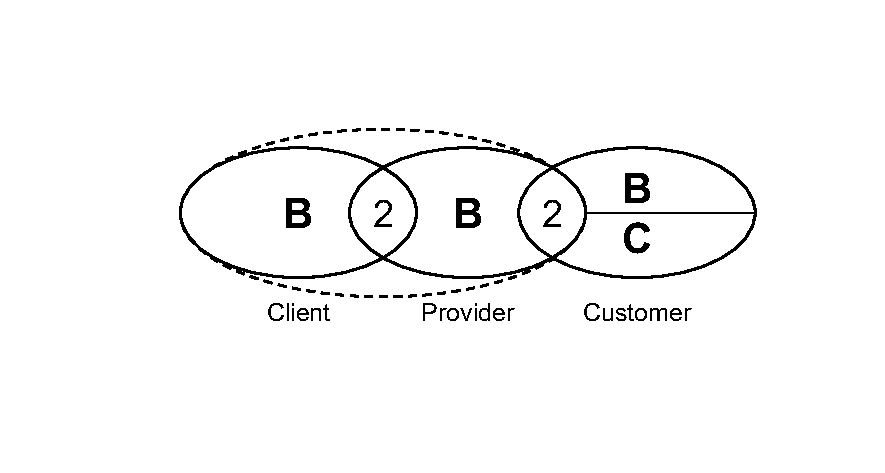
\includegraphics[width=.8\textwidth]{figures/bpochain.pdf}}
	\end{figure}

			
		\begin{itemize}
			\item process orientation  ok
			\item DEF ok 
			\item common processes that are outsourced - zahlen
			\item schewe 3: venn diagramm prozesoptimierung - bpo - outsourcing
			
			\item IT as an enabler ok 
			\item offshore, nearshore, inshore - nur nennen und auf interessante Aspekte für case eingehen
			\item Model ? Matrix ? 
		\end{itemize}
	
		\subsubsection{Parent Company}
		%% irgendwie wiederkehrende Struktur bei Parent Company und Provider...
		Motivation for outsourcing of services is based on sound economic principles, as laid out in the section about the theory of the firm. From the previously described theories explaining outsourcing, especially the economic and strategic management view applies to justify outsourcing decisions. \citeauthor{bartell1998information} names improved business focus, mitigate risks, build sustainable competitive advantage, extend technical capabilities and free resources for core business purposes \cite{bartell1998information}. Cost reduction is not included in this list (even though it was a primary driver at first), as the experience has shown that 80\% of customer service outsourcing projects aimed for cost cutting are failing \footnote{See \url{http://www.gartner.com/newsroom/id/492113}}. 
		
		cost savings argument
		
		zahlen zahlen zahlen
		
		
		\begin{itemize}
			\item reasons: focus on core competencies
			\item fields // processes no29 for India, Deloitte Outsourcing Paper
			\item challenges
			\item 
		\end{itemize}
		\subsubsection{Outsourcing Provider}
		
		\begin{itemize}
			\item dienstleistungsstruktur  : schewe
			\item no29: intro to firms, transaction costs so on
			\item no29: capabilities of Providers
		\end{itemize}
		%%%%%%%%%%
		\subsection{Customer Relationship Management}
		%%%%%%%%%%
		\enquote{A company's most precious asset is its relationship with its customers} is a quote of Theodore Levitt, Harvard Business School professor emeritus, from 1983 (LEVITT). Following this idea, marketing has undergone a shift from a brand- or product-centricity to a more customer-centered view. An absence of sharp definitions has lead to a considerable confusion in academic literature about the term customer relationship management  \cite{paynefrow2005}. 
		
		Essential terms surrounding CRM are marketing, relationship management and relationship marketing. Drawing on the taxonomy of \cite{hippnerwilde2011}, a visualization of the fundamental relationships is given in \Fig \ref{fig:crmcircles}. Under the umbrella of marketing, relationship management describes the active and systematic analysis, planning, design, selection and control of all business relationships in the sense of a holistic concept of systems, activities and goals \citep[\p{442}]{diller1995}. It has to be noted that not only relationship to customers, but also suppliers, communities, authorities, as well as internal relationship are enclosed by this term. Relationship marketing is a subset of relationship management and more strongly emphasizes customers as a target, but also comprises vertical relationships, i.e., relationships to suppliers. Within relationship marketing lies customer management or customer relationship management. Both terms are often used interchangeably by many authors \cite{Leuer2011,ryals2001customer}. This thesis therefore prefers the term customer relationship management. 
		
		
		\begin{figure}[caption={CRM in the field of marketing}, label={fig:crmcirlces}]
			{	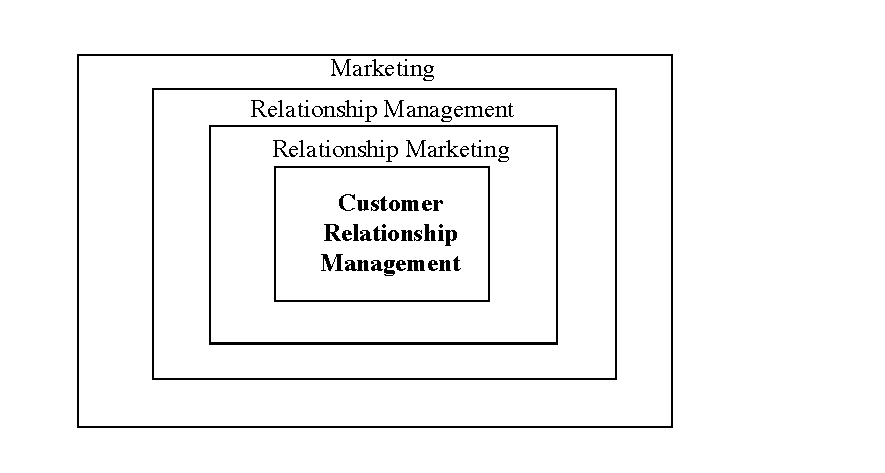
\includegraphics[width=.8\textwidth]{figures/crmcircles.pdf}}
		\end{figure}
	
		\cite{paynefrow2005} compile different standpoints and propose three views, that will be described in the following. As the name suggests, the building and sustaining of relationships to customers is always a defining characteristic of \acrshort{CRM}, but the importance of the technological component is varying. 
		
		Narrowly and tactically defined, \acrshort{CRM} refers to a technology solution and its implementation, which justifies the term's popularity in the technical field. With an increased scope, \acrshort{CRM} can be seen as the implementation of an integrated series of customer-oriented technology solutions. Widely and strategically defined, \acrshort{CRM} can be seen as a holistic approach to managing customer relationships to maximize customer value, corporate profitability, and thus, shareholder value \cite{payne2004role}. This value is realized through the developed of a relationship, that is profitable and preferably long-term. 
	
		For this thesis, a customer is defined as an individual or business that has entered the process of buying a good or service from another business. Hence, the customer has a relation to the latter, that is of interest in CRM. This relationship can be strengthened by a plethora of marketing instruments that businesses use to bind the customer. These are initiated from the businesses and directed towards the customer. The reverse way, \ie, a customer reaching to the company by considering a product is also possible.  
		
		 For establishing the communication between the two parties, two terms have emerged: channels and customer touch points\todo{src}. Channels are considered to be the more general term and from a company perspective, while a customer touch point is more specific and from the customer's view. The term channel is preferred here in contrast to customer touch points, as customer touch points are changing more rapidly and stand in contrast to the intended broad applicability of this thesis for a BPO provider. For instance, social media as a channel will likely be a long-lasting medium in CRM, while a plattform, \ie, facebook, may or may not withstand the test of time. In that sense, a channel is seen here as a more abstract type and a touch point an instance of a medium of communication between company and customer. 
		
		Communication between the customer and company can be done through a number of channels which have grown in the past years. Integration of these channels is a central task of CRM and shows increasing complexity. \cite{paynefrow2005} propose six categories: (1) sales force, (2) outlets,\ie, stores and the alike, (3) telephony, (4) direct marketing,\ie, mail, radio, television, (5) e-commerce,\ie, e-mail and internet, (6) mobile-commerce,\ie, text messaging, mobile telephony. Applying the \acrfull{MECE}-rule, one faces problems with this definition. With the advent of smart phones technology, mutually exclusion of (3),(5) and (6) is hardly possible. In addition, social networks have become increasingly important for customer interaction. This necessitates another view, which conforms to today's channel landscape and is forearmed for new channels that might emerge in future. 
		
		This thesis takes a two-dimensional views on different interaction channels in CRM. Building on the framework by \citeauthor{paynefrow2005}, the digital component gets more emphasis, as it is of striking importance today. The matrix displayed in \ref{fig:channelmatrix} positions different channels with respect to their personal or universal way of communication, as well as their orientation towards IT. The aforementioned categories (1) sales force, (2) outlets and (4) direct marketing are located in the matrix with no further change of meaning to the primary literature. Especially in the digital sphere, a more diverse view on the remaining problematic categories is taken.
		
	%			\begin{figure}[caption={Channel matrix}, label={fig:channelmatrix}]
	%		{	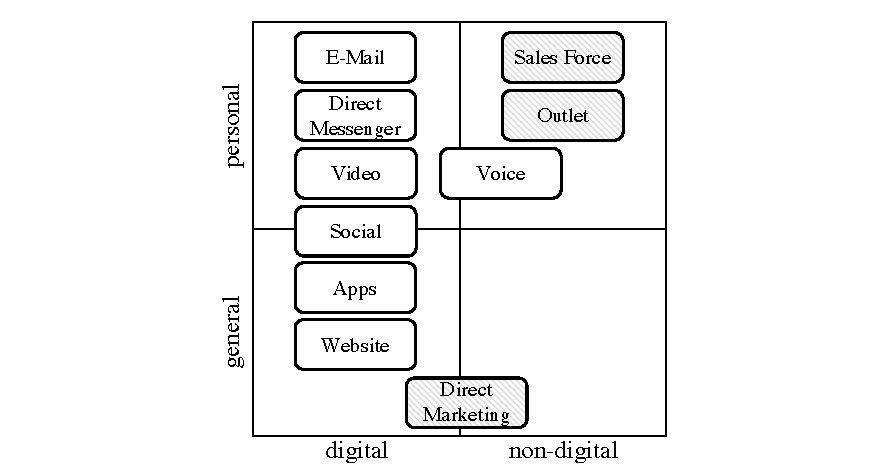
\includegraphics[width=.8\textwidth]{figures/channelmatrix.pdf}}
	%	\end{figure}
		
		EXPLOSION IN TOUCH POINTS (LEMON VORHOEF 2016).
		
		Digital channels are characterized by a strong IT-component and hence the web as an underlying technology for communication. Non-digital channels on the other hands rely on real world interaction. In general, a shift towards digital channels can be observed. For consumers they are a convenient way of communication, as their devices enable them to do interact with less effort. A stop at a retail store is more effortful than a lookup of information on the company website. Nevertheless, non-digital channels will always be part of channel portfolio, as complicated issues reason interaction with another human being face-to-face especially in the B2B-sphere. 
		
		The customer-centric view underlines the shift to personal marketing activities. This is enabled by IT and the ever increasing amounts of data that is available and possibly attributable to a single consumer. While the more personal approach is standard practice in B2B-relationships, mass media direct marketing has been the only way to target private customers in the past decades through the use of radio or television. In a data-driven world personalized relationships with consumers is an imperative to stay competitive. However, an anonymous way of retrieving information is also demanded, even though this way will likely increase the effort due to a less tailored presentation of information. 
		
		The two trends in the dimensions renders the personal / digital quadrant as an strategic priority.
		The identification of single customers is a requirement for a customer-centric view, which is only efficiently possible by information technology.  
		This again can be mapped back to the work of \citeauthor{paynefrow2005}: They name information management and multichannel integration as strategic processes. 
		
		Not every channel is used by every company. Coming from a pre-digital age, digital channels were integrated gradually and often in a heterogeneous information system landscape (chen popovich 2003). The following paragraphs shortly describe all channel categories that are not named  in  \citeauthor{paynefrow2005}. A special focus is put on customer service provision. 
		
		DEF CUSTOMER SERVICE
		INBOUND
		OUTBOUND
		SELF SERVICE
		
		
		\subsubsection{Voice}
		
		Coming from traditional, non-digital telephony, voice is a very important service channel. While non-voice channels are said to overtake by the end of 2016, it is still accounting for half of the customer service volume on its own \cite{dimensiondata2016}. However, voice is becoming more and more digital for example through \acrfull{VOIP} technology, which is one reason for the renaming. Defining characteristic is the synchronous communication and interaction with a \acrfull{CSR}. A channel's popularity is reasoned by customer's expectation to explain their problem easily(35.2\%) and get a fast response (46.4\%) according to \cite{ocm2015}. Voice is well suited here, but is also a costly option for customer service through the one-to-one interaction. \acrshort{CSR}s are not able to process multiple calls simultaneously. Outsourcing call centers has therefore become a major application across industries (SRC) as low-wage countries like India offer significant savings. 
		
		Regarding data, the shift towards digital call processing enabled the tracking of numbers, efficient routing and conversation recording for instance. Identification of callers is often possible through the caller's phone number (if not suppressed), another problem arises in outsourcing: When the client provides call routing systems and uses outsourcing as a means to process first level support for instance, the phone number might not reach the provider's systems. This renders a customer identification before start of the call impossible. Audio recordings also need to be automatically transformed into a processable format through sophisticated text-to-speech tools before using them for analytical purposes. Due to privacy reasons, these activities are restricted in many countries. 
		
		\subsubsection{E-Mail}
		
		By 2020, 50\% of the world's population is expected to have an email address \cite{radial2016}. In the developed world this number will be significantly higher. The convenience of electronic mail is the asynchronous communication from various devices, with attachments, at any time of the day and without the need to personally interact with the receiver. In customer service it is ranked second in terms of volume. 90.1\% of call centers support e-mail \cite{dimensiondata2016} today. Traditional mail or fax is included in this category, as it is plays an subordinate role: 1.4\% of customers call it their preferred channel \cite{ocm2015}. It also offers significant obstacles for customers through its slowness, costs and effort of creation and sending. 
		
		As the message content is directly processable, analytical support plays an important role in routing mails. The sender can be identified by the address, that can not be suppressed. 
		
		\subsubsection{Direct Messenger}
		
		whatsapp, social 
		\subsubsection{Video}
		
		merge with voice but digital roots. 
		Video shares several characteristics with voice: It is synchronous, two human beings are involved and the communication is based on a common spoken language. In some sense, it is voice+, as it adds the visual representation of communication partners, which is why one can argue that they will ultimately merge into one channel category. The reason for the split here is that voice has its roots in the non-digital world, while video is clearly a digital channel. It offers advantages in customer service for example through the ability to perform legally binding identification or show objects of interest live during the conversation. Adoption however remains very low //SRC, as customers need a camera in their device and the anonymity of a voice call is preferred.
		
		\subsubsection{Social}
		fb, twitter, changing
		\subsubsection{Web site}
		
		
		
	
			
		
		janina
		\subsubsection{Non-Digital Channels}
		
		janina
		
		42: stems from mid 90s, IT community. can be seen as informatin-enabled relationship marketing. 3 perspectives: narroly and tactical: implementation of a specific technology solution project. mid: implementation of a series of integrated customer-oriented tech solutions. broadly: crm is a holsitc approach to manage customer relationships to create shareholder value. channel split is old eCommerce does not make sense anymore.
		process view of payne frow helps, as it is not limited by organizational aspects. 
				\begin{itemize}
			\item CSM or CM or CRM?
			\item Value Chain - GoM PDF -- könnte man auch bei RefMod / Ordnungsrahmen machen. 			
			\item Importance for businesses
			\item characteristics, developments 
			\item payne/frow
		\end{itemize}
	
	\subsubsection{Multi-Channel CRM}
		%janina
	\subsubsection{Omni-Channel CRM}
	    %janina
	 
		%%%%%%%%%%
		\subsection{Customer Relationship Management Business Process Outsourcing Providers}
		%%%%%%%%%%
		\begin{itemize}
			\item ECIS Paper...
			\item Strategy, Capabilities from voleti concretized. 
			\item one face to the customer
			\item B2B2X
			\item virtual company
		\end{itemize}
	%%%%%%%%%%
	\section{Reference Modeling}
	\label{sec:03_refmod}
	%%%%%%%%%%
		%%%%%%%%%%
		
Conceptual models are representations of an application domain used to capture the important features to be incorporated into a specific information system (Batani et al. 1992; Bodart et al. 2001). --37 vom brocke


		\subsection{Concept}
		
		\subsubsection{The Model as a construct}
		
		
		
		\begin{itemize}
			\item kurz geschichte
			\item eigenes subheading für modellbegriff?
			\item 
		\end{itemize} 
		Reference Models can be seen as theory of information systems \cite{Schutte1998}. A model itself is defined as an "immaterial representation of an original for the purposes of a subject" \citep[\p{1}]{Becker2012Gom}. Based on the work of \cite{Stachowiak1973}, three characteristics of models are identified: mapping, reduction and pragmatism. Mapping describes the representation of natural or artificial originals, which can be models themselves. Reduction underlines the omission of certain elements of the original in a model. Pragmatism means that the selection of parts of the original is dependent on the intent of the model. Based on this notion, models of information systems (or information models in short) are explicit models that have information systems as subject matter. 
		

		and application systems, which can be put together as information systems. Information modeling, the act of creating these, is a complex task, which is why reference models are a useful means to reduce this effort \cite{Becker2007} to create application models. 
			\subsubsection{Reference Models and Application Models}
			An information model can be specified on a certain company, which is here denoted as an application model. Reference models on the other hand are not firm-specific and as the name suggests provide guidance in a defined modeling scenario. There is no accepted definition of reference model in the literature. \citeauthor{thomas2006refmod} compiles various definitions for reference models \cite{thomas2006refmod}. \citeauthor{vom2006reusable} brings in the notion of reusable conceptual models, where conceptual models are the representations of an application domain used to capture the important features to be incorporated in a specific information system \citep[\p {584}]{vom2006reusable}, as the term reference model is predominantly used in the German literature. It is agreed that a reference or application model of German understanding is a conceptual model. However it is refrained to use the terms reference conceptual model and application conceptual model over \acrfull{RM} or \acrfull{AM} . As an conceptual model's purpose is the representation of features of an information system, it is an information model. 
			
			\citeauthor{Schutte1998} puts \enquote{universal validity} and \enquote{recommending characteristics} as defining  for a reference model. Universal validity expresses that a reference model can only be valid for a class of companies, so that it can be used for creating application models. The recommending aspects states that a reference model should capture a wanted to-be state, which is in the modeler's intention. These two combined enable the wanted re-usability, which is planned by the modeler \citep[\p{36}]{vombrocke2003referenzmodellierung}. However, achieving a recommending characteristic is a subjective judgment and universal validity can always be achieved by shrinking down the target class of companies \cite{thomas2006a}. The other option, namely encompassing a large target class of companies to create \textit{one} reference model stands in contrast to practical use, as the creation of application models gets increasingly complicated the more general (and hence abstract and theoretical) \citep[\p{79}]{Schutte1998} the reference model is. Striking a balance between these trade-offs is known as the reference modeling dilemma. 
		
			For this thesis, a reference model is defined as an information model with content that is reused in the construction of other application models. The relationship between a reference and application model is characterized by reuse of reference model components in application model construction (\cf \cite{Puster2015, vombrocke2003referenzmodellierung}). 
			
			To capture the complexity in business, a data, organizational, functional or process perspective can be taken (\cf \ref{processorientation}). As only process models are subject matter in this thesis, the term process reference model is used interchangeably with reference model from here on. 
	\todo{generisches RefModVariantenmanagement}
				  %delfmann: Variantenmanagement
				  
				  
				  
				  \begin{figure}[caption={Design Process of Reusable Conceptual Models}, label={fig:refmodconst}]
				  	{	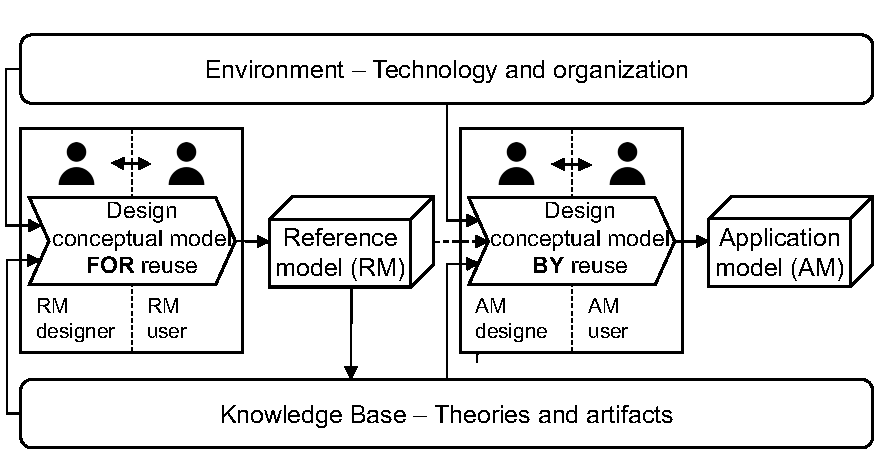
\includegraphics[width=.8\textwidth]{figures/refmodconst.pdf}}
				  \end{figure} 
				  
				  \citep[\p{587}]{vom2006reusable}
				  
			%grafik aus refmod - enzyklopädie vom brocke
		A model is created by one or multiple subjects called designers and utilized by users \cite{becker2004handelsinformationssysteme}. Model designers in context of reference modeling responsible for creating the \acrshort{RM}l itself. Their intention is to design \textit{for} reuse, \ie creating an artifact that is to be reused. The other involved stakeholder in this modeling process in the reference model user which collaborates with the designer and defines requirements for use. This first process is visualized in the left chevron in \Fig \ref{fig:refmodconst} and takes input from the knowledge base as well as the environment. The output is the  \acrshort{RM} which itself contributes to the knowledge base as an artifact. 
		
		The right chevron is similarly structured \wrt the stakeholders, but designs an application model on base of the now existing \acrshort{RM} which can be labeled as design \textit{by} reuse. Akin to the reference model designer, the application model designer takes requirements from the application model user. By doing this, the  \acrshort{AM} can represent characteristics of the application environment (\ie one organization), while still being conformable to the reference model. 
		
		\subsection{Construction}
		A construction of an \acrshort{AM} on basis of a \acrshort{RM} requires the construction of the latter beforehand. 
		\Fig \ref{fig:refmodconst} lists the knowledge base (theories and artifacts) and the environment (technology and organization) as inputs for reference modeling. For knowledge acquisition, one can differentiate in an inductive and deductive approach \cite{thomas2006mang}. Induction describes conclusions from particular cases to the general case. In this context these might be organizational settings that are observed or existing \acrshort{AM}s of organizations in the domain. Deduction infers a special from a general case and is especially employed when drawing on existing theories from the knowledge base. Loosely, these two approaches refer to the two inputs for design \textit{for} reuse in \Fig \ref{fig:refmodconst}. 
		
		The reader is referenced to \cite{Fettke2014meth} for an overview about different construction techniques. These show conformance with the design science approach \citep[\p{10}]{Puster2015} which is taken here. 
		
		
		\subsubsection{Selected Reference Models}
		
		As mentioned, a reference model is suited to fit requirements of a certain domain. The purpose of this section is to briefly present two different reference models that are used in practice: The \acrfull{SCOR} Model and the Retail-H. Both show a layer structure to manage complexity and both encompass a process reference model. 
		
		\acrshort{SCOR} allows modelling of supply chains. It is a process reference model with three detail layers. It was developed in 1996 and is now maintained by the Association for Operations Management \cite{APICS2015}. On the highest level, typically called regulatory framework, \acrshort{SCOR}  is based on six distinct management processes: Plan, Source, Make, Deliver, Return and Enable. While the regulatory framework assists in defining scope, the second configures the type of supply chain (Make-to-Order, Build-to-Order, Engineer-to-Order). On the thirds level these are decomposed into generic process steps (e.g., issue product). Even more detailed processes are considered company specific and therefore no part of the model. Furthermore, performance metrics are also defined on each level. 

		\begin{figure}[caption={SCOR Model}, label={fig:scor}]
		{	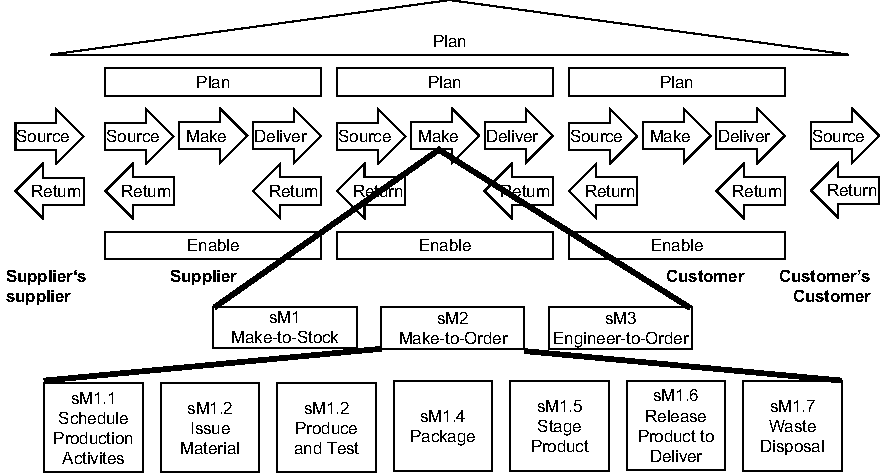
\includegraphics[width=.8\textwidth]{figures/scor.pdf}}
		\end{figure}
	

		In the domain of retail, the Retail-H is a reference model that includes process, function and data models. Developed by \cite{Becker2004a}, it has been adapted to suit special segments of the domain \footnote{for instance eCommerce, Central Clearance, Central Settlement. \cf \cite{Puster2015}}. 
		It is structured with four layers of detail: the regulatory framework, main processes, detail processes and process building blocks. The core of the regulatory framework is made up of three parts that form the H (a connection to the German word for retail: \enquote{Handel}). While the left part of the H describes the supply side, the right covers the distribution side. Both are connected through logistics. All of these core processes are business processes, the roof and foundation consist of support processes thereby making use of the framework reference design as proposed in \cite{Meise2001} while simultaneously capturing domain-specific aspects in the set-up of the framework. 
		Each segment on the regulatory framework is a main process, that has several main process steps and each of these is a detail process. The detail process steps are process building blocks and show the highest level of detail. 
		\begin{figure}[caption={Retail-H}, label={fig:retailh}]
			{	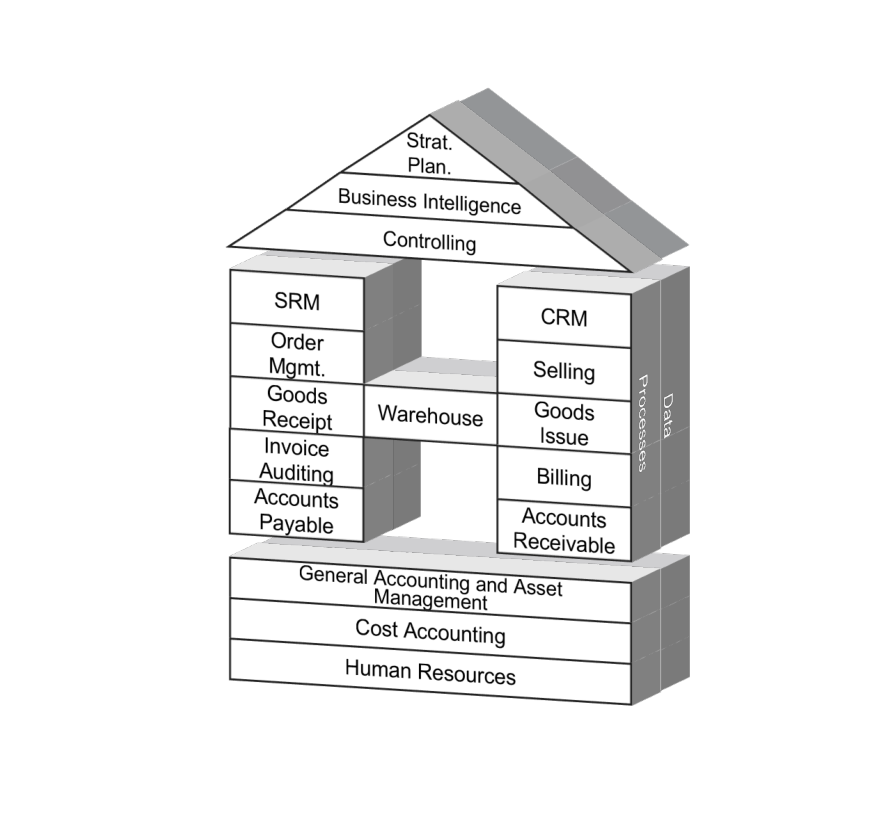
\includegraphics[width=.6\textwidth]{figures/retailh.pdf}}
		\end{figure}
		

		%%%%%%%%%%

		%%%%%%%%%%
		\subsection{Benefits}
		%%%%%%%%%%
		\begin{itemize}
			\item  ECIS paper part!
			\item TODO: Fragen ob man hier schon auf bpo crm aspekte eingeht... eigentlich schon. was bringen die allgemeinen denn. 
			\item auch vom Brocke checken 
		\end{itemize}
		%%%%%%%%%%
		\subsection{icebricks as a Process Modeling Language}
		
	 Fundamental for a language is the ability to communicate through use of it (SRC). While reference models are formulated in various languages, several options may arise. There are reference models like \acrshort{SCOR}, which avoid the use of a defined modeling language to ensure wide industry adoption through not interfering with used modeling languages. However, this necessitates an increased complexity in adoption, as an application within a company requires the translation into a sound process modeling language. While the framework level does not need to comply to a formalized language, more detailed layers of the reference model without clearly defined syntactical guidance increase the risk of misunderstanding among users.
	 This reasons the choice of using a defined process modeling language for this undertaking.
	 
	 The next step is to decide what language to use. Traditional modeling languages like EPCs, Petri-Nets or BPMN show similarities. Being syntactical languages, they offer large degrees of freedom in usage. What might look like an advantage at first sight, turns out to be disadvantageous. As process management approaches have increased number and variety of model designers and users enormously, more and more non-experts get in contact with process models and thus create models of less quality. The definition of modeling conventions becomes necessary to help the modeler to conform certain standards. A way to confront this challenge are the \acrfull{GOM} \cite{BeckerGOM2012}, which are an analogy to the \acrfull{GAAP}. However, conforming to these guidelines will lead to increased resource requirements in these undertakings. Semantic process modeling languages avoid this by enforcing additional rules that models have to follow. icebricks \cite{becker2015icebricks} is one example that realizes this concept and has been used for reference modeling. In addition to syntactical correctness, \ie conforming to the language's meta model, other aspects are also considered which would otherwise be taken care of by combining \acrshort{GOM} and syntactical languages. Because the additional check for guideline compliance is unnecessary in semantic languages, they are more efficient. After a short summary of the language,  the \acrshort{GOM} are described and it is argued why icebricks conforms to the aspects. 
	 
	 icebricks has a four layer architecture, which consists of four layers of abstraction: (1) process framework, (2) main process, (3) detail process and (4) process building blocks. Each lower layer is an element of the higher layer, i.e. an element on the framework layer is a main process. Each part of a main process is a detail process and so on. A glossary ensures unambiguous terminology and meaning of processes, especially important for providers with a decentralized structure as well as to manage client vocabulary. Variants are integrated in the layer concept, so that every main or detail process can have different variants to model different peculiarities within a process. One example can be the three variants make-to-stock, make-to-order or make-to-engineer as variants of a production process. 
	 
	 
	 \subsubsection{Correctness}
	 Correctness can be seen from a semantical and syntactical point of view. The latter can be assured when the model conforms to a meta-model of the language, which is shown in \ref{fig:icebricksmetamodel}. On the other hand, semantical correctness refers to the correct display of content inside the model. This correctness is hard to prove, but can be supported by a clear and simple structure that minimizes misunderstanding (which negatively impacts semantical correctness). While the other named languages tend to generate very complex models, the strict four layer structure of icebricks limits model complexity. 
	 
	 	 \begin{figure}[caption={icebricks meta model}, label={fig:icebricksmetamodel}]
	 	{	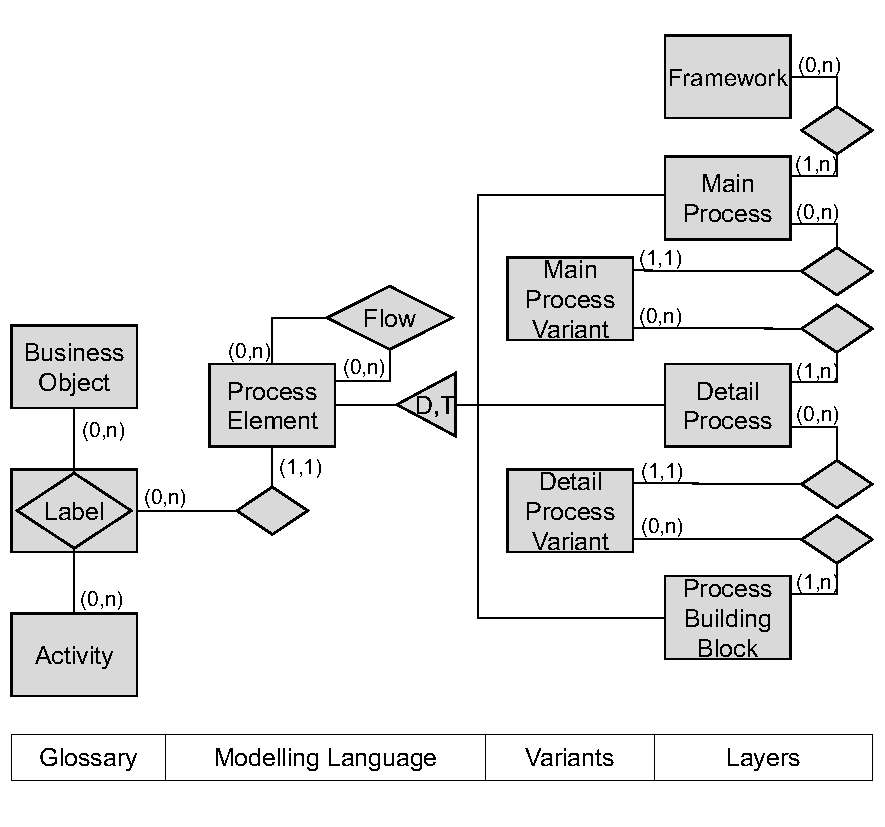
\includegraphics[width=.8\textwidth]{figures/icebricksmetamodel.pdf}}
	 \end{figure} src püster
 
	 \subsubsection{Relevance}
	 Relevance refers to the depiction of elements inside the model, which are necessary for the modeling purpose. This causes two boundaries: On the one hand, no element should be included in the model that has no connection to the real world. On the other hand, no aspect of the real world should be part of the model, which does not comply with the modeling purpose. Again, a simple structure of processes helps to guide the modeling procedure. 
	 
	  \subsubsection{Economic efficiency}
	 Syntactical languages are more error prone than semantical languages, because defects occur a posteriori, \ie, after modeling. As a semantical language ensures more guidance and strictness to its modeler, less errors exist in the model because they are identified during model creation. This reduces corrections on the outcome, which benefits the economic goal of successfully creating a model for the intended purpose with minimal effort (efficiency). In addition, icebricks as a reference modeling language has the ability to translate into other languages, because it only uses activities and control flow on every level. This enables a more efficient application of the reference model in companies. 
	 
	 \subsubsection{Clarity}
	 Clarity aims at a clear structure within a model and a simple navigation through different process models. The four layer approach, variant modeling and limited use of branches addresses a clear and consistent structure in an icebricks process model. Furthermore, the glossary ensures a labeling of processes, that conforms to the proposed verb + object construct \cite{7pmg} and tackles the problem of naming conflicts.
	 
	 \subsubsection{Comparability} 
	 With respect to different modeling languages, comparability describes the transfer of content inside a model in language A to another language B without sacrificing information. icebricks was designed to provide this ability, as the application of a reference model in multiple companies consequently leads to contact with different process modeling languages. 
	 
	 \subsubsection{Systematic Design}
	 The scope of reference models necessitates different layers of detail to manage complexity. Consistence between different layers is a challenge when separate models are built for each layer. By applying a layer structure, variant modeling and the use of a glossary, icebricks guides the modeler during model creation to create well-structured models in the first place. 

	
